\mychapter{Scale}{Scale}
\begin{figure}[h]
  \begin{minipage}[t]{0.45\textwidth}
    \fbox{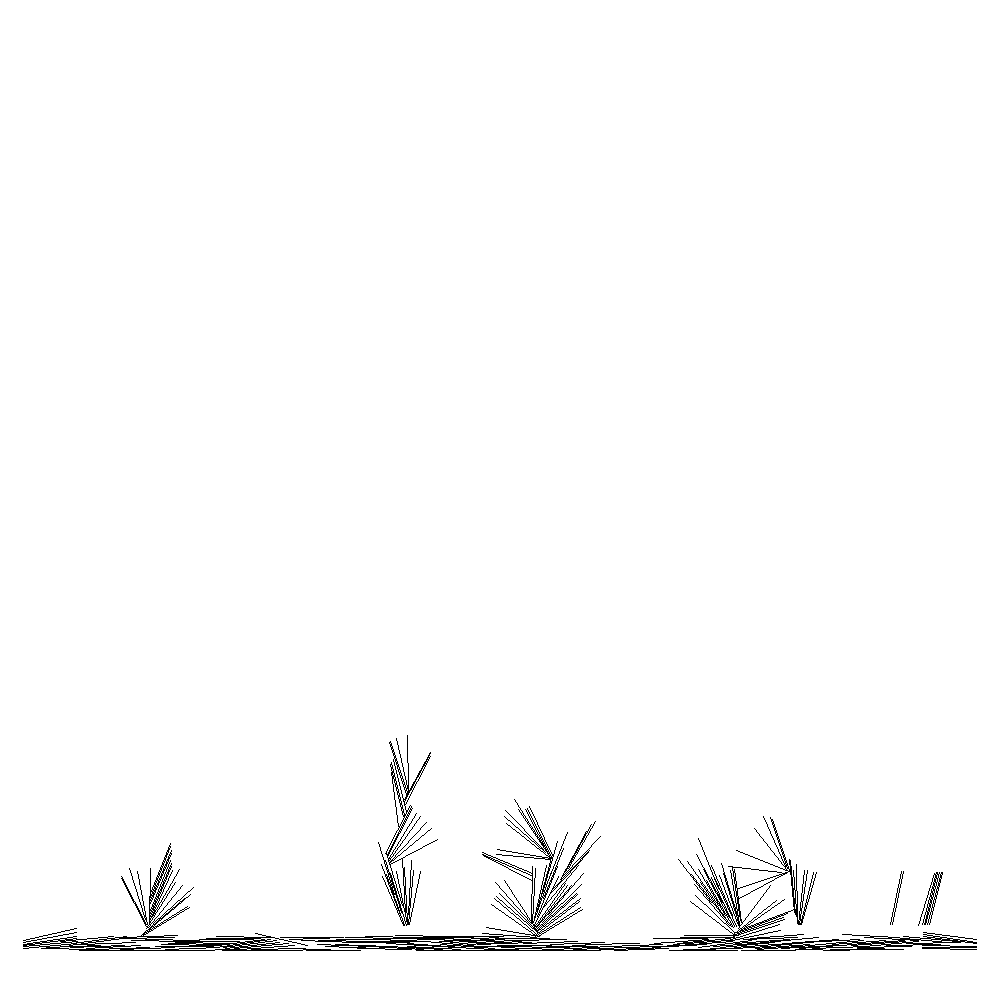
\includegraphics[width=\textwidth]{data/sca_comp1_L.png}}
  \end{minipage}
  \hfill
  \begin{minipage}[t]{0.45\textwidth}
    \fbox{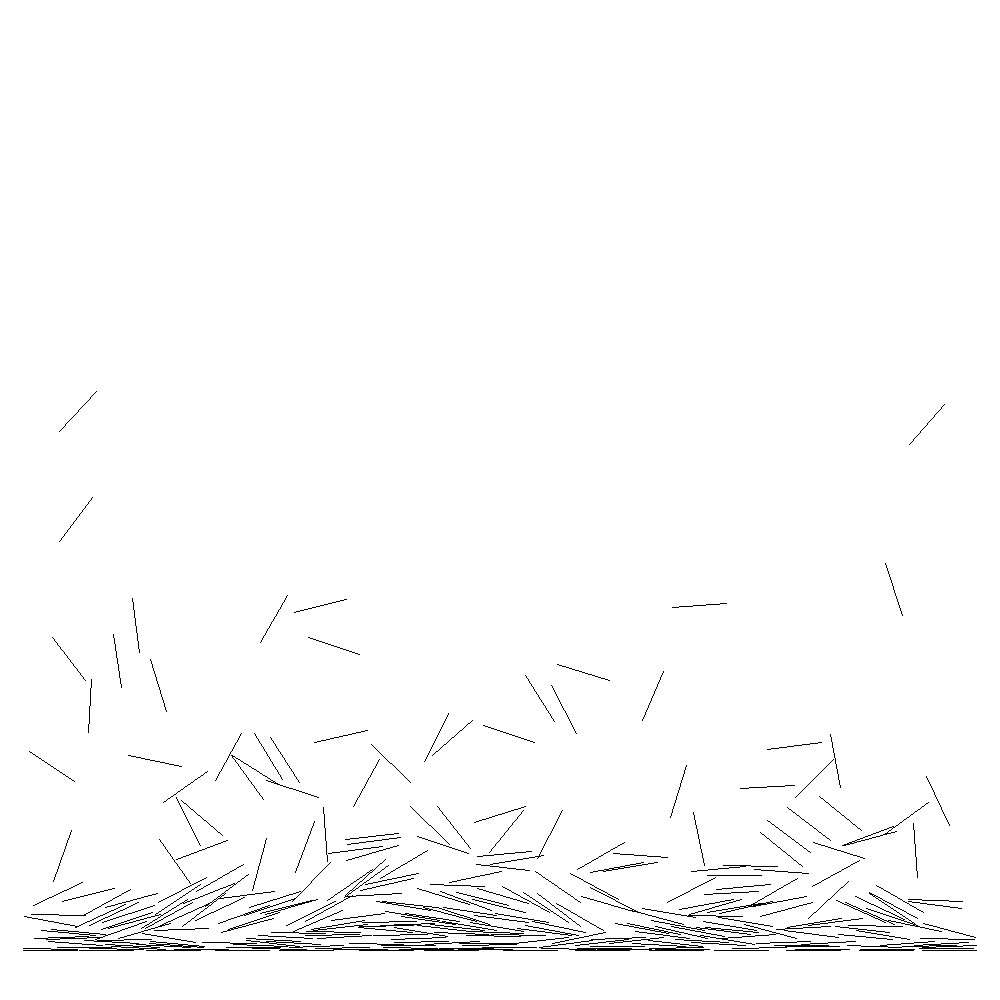
\includegraphics[width=\textwidth]{data/sca_comp1_R.png}}
  \end{minipage}
  \caption{Comparison of scales 5e-3 (left) and 5e-5 (right). We can see how after 5e8 iterations the particles just settle out for the larger scale, however they do tend to bind and form trees. For the smaller scale, the particles do align better, but do not sink down and instead just float with random movements.}
  \label{fig:sca_comp1}
\end{figure}
The size of the domain or the scale of the system $s$ has a large influence on the system. First of all, it controls the time scales at which movements happen, and secondly it controls the influence of gravity on the particles.
The diffusion parameters directly depend on the scale of the system. The timescales, as given implicitly by the diffusion coefficients, are of the following orders
\begin{equation}
  \begin{array}{RLL}
    D_\| = O\kfrac{\ln s}{s},\\
    D_\perp = O\kfrac{\ln s}{s},\\
    D_r = O\kfrac{\ln s}{s^3}.\\
  \end{array}
\end{equation}
Hence the ratio of rotational to transversal movement increases as the scale decreases. This results in differing pattern formations:
For small scales the rods are more likely to reorder themselves such that the orientation of neighbouring rods is very similar. For larger scales the rods do not reorder themselves and therefore many rods with largely varying orientations collide frequently and only slightly reorder themselves over time. This results in interlocking between rods and creates tree-like structures.\\
For large scales the interlocking is amplified by the increased gravity of particles. Due to the higher potential energy differences for small height-movements, the Metropolis-Hastings algorithm has a much lower acceptance rate for upward movements. This combined with less rotational movement creates structures which either do not resolve themselves at all or only do so very slowly. For small scales the reduced gravitation means that the acceptance rate for upward movements is almost equal to the acceptance rate of downward movements. This results in sedimentation at the bottom as well as the top of the domain, and also leaves particles floating in the center which will not sediment at all.\\
\cite{SED} does not give the results for either small or large scales, their results do neither show the formation of tree like structures nor the limited sedimentation at the top and on the bottom of the domain. For medium scales we get similar results, but these require a large fine-tuning effort.
\begin{figure}[h]
  \begin{minipage}[t]{0.45\textwidth}
    \hspace{-0.1\textwidth}
    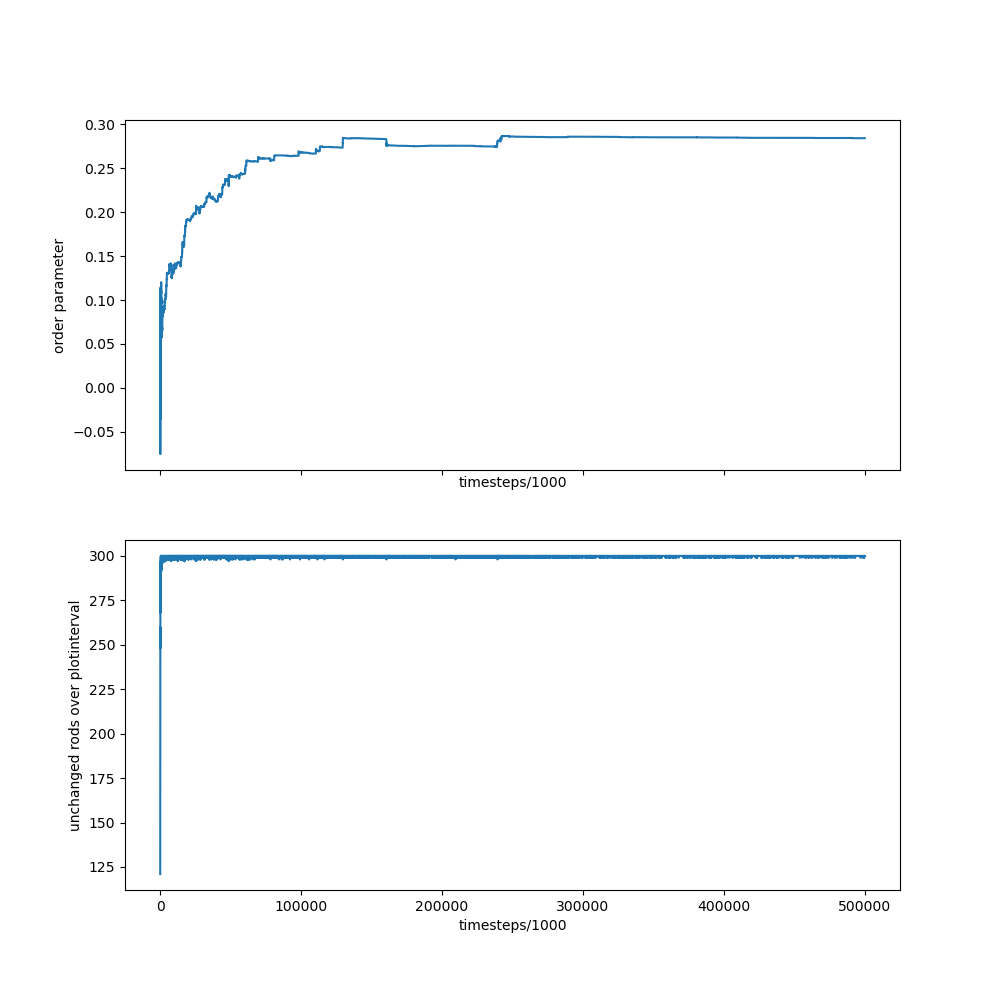
\includegraphics[width=1.2\textwidth]{data/sca_comp2_L.png}
  \end{minipage}
  \hfill
  \begin{minipage}[t]{0.45\textwidth}
    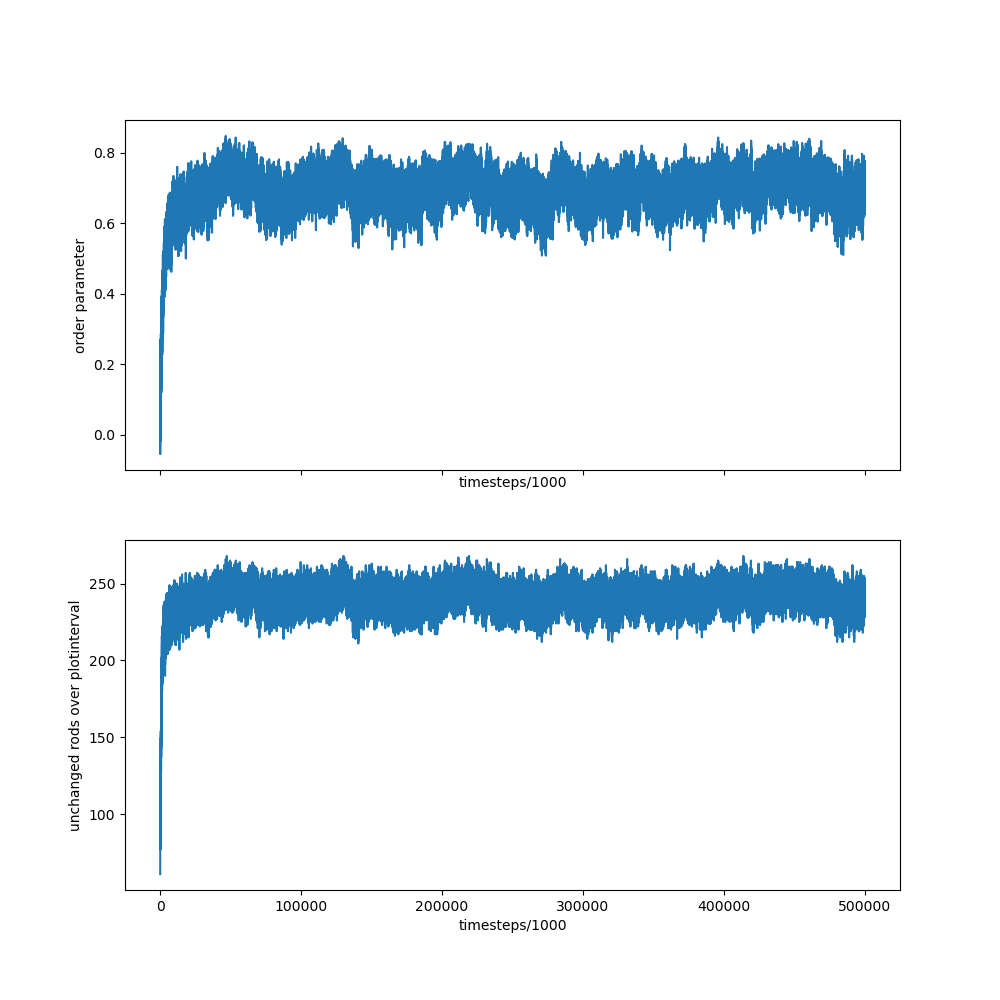
\includegraphics[width=1.2\textwidth]{data/sca_comp2_R.png}
  \end{minipage}
  \caption{Comparison of scales 5e-3 (left) and 5e-5 (right). While the order parameter(upper graph) for the scale 5e-3 shows normal ordering as we expect, for the smaller scale of 5e-5 we see a lot of noise and randomness in the order parameter. This is due to the lack of sedimentation/weaker gravitational force. Something similar can be seen in the number of unmoved particle diagrams below: On the left, it converges fast as we expect of interlocking and tree building systems. On the right, we have a lot of randomness in that signal, as the rods are not locked up in any way and keep rotating.}
  \label{fig:sca_comp2}
\end{figure}
\clearpage
